% ---------------------------------------------------------------------------
% ---------------------------------------------------------------------------
% Modelo LaTex para preparação do documento final de Dissertação de Mestrado
% O modelo está em conformidade com ABNT NBR 14724:2011: 
% Programa de Pós-Graduação em Ciência da Computação
% Universidade Federal do Piauí
% Versão: v0.9
% ---------------------------------------------------------------------------
% ---------------------------------------------------------------------------

\documentclass[
	% -- opções da classe memoir --
	%article,
	12pt,					% tamanho da fonte
	%openright,				% capítulos começam em pág ímpar (insere página vazia caso preciso)
	oneside,					% para impressão em verso e anverso. Oposto a oneside
	a4paper,					% tamanho do papel. 
	]{memoir} %abntex2
	
% ---------------------
% Pacotes OBRIGATÓRIOS
% ---------------------
\usepackage{lmodern}				% Usa a fonte Latin Modern			
\usepackage[T1]{fontenc}			% Selecao de codigos de fonte.
\usepackage[utf8]{inputenc}			% Codificacao do documento (conversão automática dos acentos)
\usepackage{lastpage}				% Usado pela Ficha catalográfica
\usepackage{indentfirst}			% Indenta o primeiro parágrafo de cada seção.
\usepackage{hyperref} 				% controla a formação do índice
\usepackage{graphicx}	       		% Inclusão de gráficos
\usepackage{epsfig,subfig}			% Inclusão de figuras
\usepackage{microtype} 				% Melhorias de justificação
% ---------------------
		
% ---------------------
% Pacotes ADICIONAIS
% ---------------------
\usepackage{lipsum}						% Geração de dummy text
\usepackage{amsmath,amssymb,mathrsfs, amsthm}	% Comandos matemáticos avançados 
\usepackage{setspace}  					% Para permitir espaçamento simples, 1 1/2 e duplo
\usepackage{verbatim}					% Para poder usar o ambiente "comment"
\usepackage{tabularx} 					% Para poder ter tabelas com colunas de largura auto-ajustável
\usepackage{afterpage} 					% Para executar um comando depois do fim da página corrente
\usepackage{url} 						% Para formatar URLs (endereços da Web)
\usepackage{todonotes}  				% Lista de afazeres To-dos
\usepackage{longtable}					% Tabela que ocupam mais de uma página
\usepackage{booktabs}					% Melhora o estilo das tabelas
\usepackage{float}						% Outras opções para ambientes flutuantes
\usepackage{pagecolor}					% Controlar a cor da página
% ---------------------

% ---------- Babel e ajustes -------------
\usepackage[brazil]{babel}		% idiomas
\addto\captionsbrazil{
	%% ajusta nomes padroes do babel
	\renewcommand{\bibname}{Refer\^encias}
	\renewcommand{\indexname}{\'Indice}
	\renewcommand{\listfigurename}{Lista de ilustra\c{c}\~{o}es}
	\renewcommand{\listtablename}{Lista de tabelas}
	%% ajusta nomes usados com a macro \autoref
	\renewcommand{\pageautorefname}{p\'agina}
	\renewcommand{\sectionautorefname}{se{\c c}\~ao}
	\renewcommand{\subsectionautorefname}{subse{\c c}\~ao}
	\renewcommand{\paragraphautorefname}{par\'agrafo}
	\renewcommand{\subsubsectionautorefname}{subse{\c c}\~ao}
	\renewcommand{\paragraphautorefname}{subse{\c c}\~ao}
} 

% Definir a cor das páginas
%\definecolor{ft}{HTML}{fff1e0}

% ---------------------
% Pacotes de CITAÇÕES
% ---------------------
\usepackage[brazilian,hyperpageref]{backref}	% Paginas com as citações na bibl
\usepackage[alf]{abntex2cite}				% Citações padrão ABNT (alfa)
%\usepackage[num]{abntex2cite}				% Citações padrão ABNT (numericas)
% ---------------------

% O tamanho da identação do parágrafo é dado por:
\setlength{\parindent}{1.3cm}
% A identação e margens de itemizações deve ser igual ao parágrafo
\setlength{\leftmargini}{1.7cm}

% Controle do espaçamento entre um parágrafo e outro:
\setlength{\parskip}{0.2cm}  % tente também \onelineskip

% ---------------------
% Compila o indice
% ---------------------
\makeindex
% ---------------------

%------------------------------------------------------------------------
% diretiva includeonly enquanto escreve o texto por capítulos
%\includeonly{capitulos/introducao}
%\includeonly{capitulos/fama}
%\includeonly{capitulos/grossman}
%\includeonly{capitulos/comportamental}
%\includeonly{capitulos/testes}
%\includeonly{capitulos/conclusao}

\title{Hipótese de Mercados Eficientes: \\teoria e testes}
\author{Gabriel Dias Medeiros Pereira \and Rafael Felipe Bressan}
\date{28 de junho de 2018}

%%%%%%%%%%%%%%%%%%%%%%%%%%%
%%  INICIO DO DOCUMENTO  %%
%%%%%%%%%%%%%%%%%%%%%%%%%%%
\begin{document}
	\maketitle
	
	\pagenumbering{roman}
% ---------------------
% Compila a lista de afazeres
% ---------------------
%
%\listoftodos
% ---------------------

% Retira espaço extra obsoleto entre as frases.
%\frenchspacing

% Ajusta a cor da página
%\pagecolor{ft}

% Lista de ilustrações
%\pdfbookmark[0]{\listfigurename}{lof}
%\listoffigures*
%\cleardoublepage

% Lista de tabelas
%\pdfbookmark[0]{\listtablename}{lot}
%\listoftables*
%\cleardoublepage

% Inserir o SUMÁRIO
\newpage
\pdfbookmark[0]{\contentsname}{toc}
\tableofcontents*
\cleardoublepage

% ----------------------------------------------------------
% ELEMENTOS TEXTUAIS (Capítulos)
% ----------------------------------------------------------
%\textual
% Elementos textuais com numeração arábica
\pagenumbering{arabic}
% Reinicia a contagem do número de páginas
\setcounter{page}{1}

% Inclui cada capitulo da Dissertação

\chapter*[Introdução]{Introdução}
\addcontentsline{toc}{chapter}{Introdução}
\label{chap:Introdução}
A suposição que os mercados seriam informacionalmente eficientes ronda a teoria financeira desde o início do século 20, onde se cogitava que o preço das ações de empresas flutuavam aleatoriamente. A pesquisa sobre se os investidores podem prever com sucesso os preços das ações tem raízes na tese de doutorado de Louis Bachelier, "A Teoria da Especulação" em 1900. Este foi o primeiro esforço a empregar teoria, incluindo técnicas matemáticas e estatísticas para explicar por que o mercado de ações se move da forma como o faz.

Bachelier derivou uma fórmula que explicava o hoje conhecido movimento Browniano, o qual descreve o comportamento de partículas sujeitas a choques aleatórios no espaço.Também desenvolveu o conceito largamente utilizado de processos estocásticos, a análise de movimentos aleatórios entre variáveis estatísticas. Além disso, ele fez a primeira tentativa de precificar instrumentos financeiros como opções e futuros. E ele fez tudo isso em um esforço para explicar porque os preços nos mercados de capitais são impossíveis de prever.

Com o passar do tempo, o movimento browniano passou a ser chamado de passeio aleatório na literatura sobre finanças. Ninguém sabe quem usou essa expressão pela primeira vez, mas se tornou cada vez mais familiar entre os acadêmicos durante a década de 1960. 

A literatura econômica mais recente se inicia com \citeonline{Muth1961} que introduz a teoria de expectativas racionais. Samuelson em 1965 publica um artigo com o título, "Proof that Properly Anticipated Prices Fluctuate Randomly".Em um mercado que apresente eficiência de informação, o preço das ações deve se mover de acordo com um passeio aleatório. Antes do advento das expectativas racionais, os economistas acreditavam que as expectativas eram formadas com informações passadas das variáveis a serem previstas, a esta teoria se chamam expectativas adaptativas.

As expectativas adaptativas foram criticadas pelo fato de as pessoas usarem mais informação do que apenas dados passados em uma única variável para formar suas expectativas desta, elas usam todas as informações relevantes e disponíveis para tanto. Além disso, as pessoas muitas vezes mudam suas expectativas rapidamente à luz de novas informações. Para atender a essas objeções às expectativas adaptativas, John Muth desenvolveu sua teoria de expectativas racionais, que pode ser declarada da seguinte maneira: \emph{as expectativas serão idênticas às previsões ótimas usando todas as informações disponíveis.}

Eugene Fama, conhecido acadêmico e pesquisador do mercado financeiro, tornou-se um dos mais eloquentes propagadores da hipótese de mercados eficientes durante a década de 1960. Sua ideia de um mercado eficiente assim se resume: \emph{"Um mercado no qual os preços sempre refletem completamente todas as informações disponíveis, é chamado de eficiente"}. Esta ficaria conhecida como a forma forte de eficiência nos mercados.

Burton G. Malkiel mais recentemente faz uma definição mais ampla: \emph{"Um mercado de capitais é dito eficiente se este completa e corretamente reflete toda a informação relevante em determinar o preço dos ativos. Formalmente, o mercado é dito eficiente com relação a um conjunto de informação (\ldots) se os preços não forem afetados pela revelação daquela informação para todos os participantes. Ademais, eficiência com relação a um conjunto de informação (\ldots) implica que é impossível obter lucros econômicos ao se operar com base neste conjunto de informação"}.

A principal implicação da hipótese de mercados eficientes - HME, a partir de agora, é que os investidores não podem obter retornos ajustados ao risco além daqueles oferecidos pela carteira de mercado de forma consistente. E por quê não? A competição entre os muitos agentes em busca de lucros elimina qualquer escolha óbvia. A administração ativa de portfólios é um jogo de soma zero mesmo antes dos custos envolvidos, após estes custos e taxas de administração, passa a ser um jogo de soma negativa. De fato, diversas análises empíricas confirmam que a maioria dos administradores tem um desempenho inferior aos índices passivos após as taxas. Essa busca incessante pelo lucro nos mercados faz com que as possibilidades de lucros extraordinários sejam eliminados através de uma espécie de "arbitragem". Os agentes compram aquelas ações que possuem expectativas de lucros maiores e vendem aquelas menos favorecidas. Este movimento faz com que as ações com forte demanda tenham seus preços elevados, e portanto, seus prospectos de retorno futuro diminuídos. O inverso ocorre para as ações de baixa procura. Deste modo, todos os ativos no mercado acabam por oferecer retornos ajustados ao risco equivalentes ao mercado como um todo.

Isso não significa que o mercado esteja sempre correto. De fato, nada na HME ou mesmo na teoria das expectativas racionais, afirma que os agentes não possam estar errados em suas previsões. Como o preço de um ativo financeiro pode ser dado pelo valor presente descontado de todos os fluxos de caixa futuros e ninguém pode prever com precisão esses fluxos futuros e, portanto, os preços de mercado devem estar sempre errados. Os mercados podem ser eficientes, mesmo que às vezes cometer erros notórios na avaliação, como fizeram durante a bolha da Internet. Os mercados podem ser eficientes mesmo se muitos participantes do mercado forem bastante irracionais e se os mercados forem frequentemente fortemente influenciados pela psicologia.

Durante vários anos, o foco principal da pesquisa sobre os mercados de capitais foi determinar se o passeio aleatório é ou não uma descrição válida dos movimentos dos preços de ativos financeiros, como uma forma de testar a hipótese de mercados eficientes.

Mais recentemente com o advento da teoria comportamental nas finanças, o foco passou a ser em buscas de retornos anormais e previsíveis que contraponham-se a HME. Um dos primeiros trabalhos sobre anomalias de retorno a longo prazo é \citeonline{Bondt1985}. Quando as ações são classificadas em com base em retornos passados de três a cinco anos, os vencedores anteriores tendem a ser perdedores futuros e vice-versa. Eles atribuem essas reversões de retorno de longo prazo à reação exagerada do investidor. De Bondt e Thaler argumentam que a reação exagerada à informação passada é uma previsão geral da teoria da decisão comportamental de \citeonline{Kahneman1982}. Assim, pode-se levar a reação exagerada para a previsão de uma alternativa financeira comportamental à eficiência do mercado. Na maior parte, entretanto, a literatura sobre anomalias não dispõe de uma hipótese alternativa a HME.

Se a reação exagerada fosse o resultado geral em estudos de retornos de longo prazo, a eficiência do mercado estaria morta, substituída pela alternativa comportamental. Entretanto, parecem haver tantos estudos que identificam pouca reação dos mercados quanto sobre-reação. Por exemplo, o efeito momento, identificado por \citeonline{Jegadeesh1993} onde as ações com altos retornos durante o último ano tendem a ter retornos elevados nos próximos três a seis meses. Ou seja, é possível obter retornos superiores seguindo uma regra fixa, evidência de sub reação do mercado que proporciona retornos anormalmente altos.



\chapter{As Versões de Eficiência}
\label{cap:fama}

A hipótese de mercados eficientes (HME) vem evoluindo desde a década de 1960, da teoria do passeio aleatório para os preços dos ativos para a hipótese de mercados eficientes em suas formas forte, semi-forte e fraca advogada por Eugene Fama na década de 1970, a quase-eficiência de Grossman e Stiglitz na presença de custos de transação até a crítica comportamentalista mais recentemente.

A HME em sua formulação mais conhecida deve-se a Fama e foi desenvolvida na década de 1960 para então ser popularizada e ganhar adesão acadêmica através de seu influente artigo "Efficient Capital Markets", \citeonline{Fama1970}.

Em sua revisão de 1970, Fama distingue três formas diferentes da
HME.

\begin{enumerate}
	\item A forma “fraca” afirma que toda a informação sobre preços está integralmente refletida nos preços correntes dos ativos, no sentido de que as mudanças de preços atuais não podem ser previstas a partir de preços passados. 
	\item A forma “semi-forte” exige que o preço do ativo mude para refletir integralmente todas as informações publicamente disponíveis e não apenas os preços passados.
	\item A forma “forte” que postula que os preços reflitam totalmente as informações, mesmo que algum investidor ou grupo de investidores tenha acesso exclusivo a alguma informação.
\end{enumerate}

Fama considerava a forma forte de eficiência como \emph{benchmark} para as demais formas de eficiência e na prática, não era alcançável. Entretanto, para a forma fraca ele conclui naquele artigo que havia fortes evidências empíricas em favor desta hipótese.

Em 1991 Fama fez uma segunda revisão sobre a HME, \citeonline{Fama1991}. Nesta época já havia ficado claro que a distinção entre as formas fraca e semi-forte de eficiência dos mercados eram redundantes. O modelo de passeio aleatório para os preços também havia sido fortemente atacado e parecia não mais se sustentar, \citeonline{Lo1988}.

Um grande número de estudos na literatura financeira confirmou que
os retornos das ações em diferentes horizontes (dias, semanas e meses) podem ser previstos em algum grau por meio de taxas de juros, retorno de dividendos e uma variedade de variáveis macroeconômicas e exibiam claras variações durante o ciclo de econômico. Vários estudos também mostraram que os retornos tendem a ser mais previsíveis quanto mais longo o horizonte de previsão e menor a frequência dos retornos utilizados.

Como o próprio Fama em sua segunda revisão da HME em 1991 notou, um teste para a hipótese de mercado eficiente necessariamente envolve um teste conjunto. Eficiência de mercado e o modelo utilizado para precificação dos ativos. A rejeição da hipótese nula de mercados eficientes pode se dar portanto, em função de o mercado realmente não ser eficiente ou o modelo de precificação utilizado não estar corretamente especificado. Fama conclui que "portanto, eficiência de mercado \emph{per se} não é testável".

No centro da HME estão as três premissas básicas a seguir:

\begin{enumerate}
	\item Racionalidade do investidor: supõe-se que os investidores são racionais, no sentido de que atualizam corretamente suas crenças quando novas informações estão disponíveis. Mesma base das expectativas racionais.
	\item Arbitragem: as decisões de investimento individuais satisfazem a condição de arbitragem, não devem existir lucros potenciais que não tenham sido explorados.
	\item Racionalidade coletiva: os erros aleatórios dos investidores se anulam no mercado. Isso requer que erros individuais devem ser transversalmente independente ou pelo menos apenas fracamente correlacionados.
\end{enumerate}

A hipótese das expectativas racionais é bastante forte, e é improvável
que se mantenha em todos os momentos em todos os mercados. Mesmo que se assuma que no mercado financeiro o processo de aprendizagem e descoberto do preço "correto" ocorra razoavelmente rápido, ainda haverá períodos de turbulência onde os participantes do mercado estarão procurando no escuro, tentando e
experimentando diferentes modelos para os retornos em excesso aquele livre de risco e frequentemente com desvios marcantes
dos resultados racionais comuns. O comportamento de manada e a alta correlação entre os participantes do mercado também podem
levar a desvios da solução de equilíbrio sob expectativas racionais.

Fricções de mercado (i.e. custos de transação ou aquisição de informações) provém outras fontes de previsibilidade do mercado, e portanto, de ineficiências aparentes destes. Estas fricções introduzem um distanciamento entre a correta previsão dos preços e a média de sua estimativa feita pelos agentes de mercado. Em outras palavras, mesmo que os agentes formem suas expectativas racionalmente, estes são impedidos pelas fricções de atuarem no mercado até a completa exaustão da possibilidade de arbitragem, e portanto, os preços correntes refletem as informações disponíveis somente até o limite onde existe lucro a ser obtido descontados os custos de transação e aquisição das informações. Isto faz com que os preços futuros possam ser previstos, muito embora não possam ser economicamente explorados, e o mercado não é eficiente.

\chapter{Quase Eficiência}
\label{cap:grossman}

Sanford J. Grossman e Joseph E. Stiglitz, \citeonline{Grossman1980}, mostraram que é impossível para um mercado ser perfeitamente eficiente em termos de informação. Como as informações são dispendiosas, os preços não podem refletir perfeitamente as informações disponíveis, pois, se o fizessem, os investidores que gastassem recursos na obtenção e na análise não receberiam remuneração. Assim, um modelo sensato de equilíbrio de mercado deve deixar algum incentivo para a coleta de informações. Nas palavras dos autores os mercados devem apresentar "oportunidades de lucro suficientes, ou seja, ineficiências, para compensar os investidores pelo custo de negociação e coleta de informações."

Apenas no caso extremo e irreal, onde todas as informações e custos de negociação são zero, seria de se esperar que os preços refletissem totalmente todas as informações disponíveis. Mas se a informação é, de fato, sem custo, ela seria conhecida mesmo antes de os preços de mercado serem estabelecidos.

Como Fama reconheceu uma versão mais fraca e economicamente mais sensata de hipótese de eficiência seria necessária, ou seja, “os preços refletem as informações ao ponto em que os benefícios marginais de agir sobre a informação (os lucros a serem feitos) não excedem os custos marginais". Isso, por sua vez, torna a tarefa de testar a eficiência do mercado ainda mais complicada e exigiria modelos de precificação de ativos em equilíbrio que permitissem informações e custos de negociação em mercados com muitos agentes diferentes e com crenças não convergentes.

Diante dessas dificuldades, alguns defensores da HME optaram por uma noção baseada no comércio e definiram os mercados como eficientes, se não fosse possível para os investidores "obter retornos acima da média sem aceitar riscos acima da média", \citeonline{Malkiel2003}. Essa noção pode levar em conta informações e custos de transação e não envolve testar hipóteses conjuntas. Mas isso está muito distante da ideia básica de mercados como alocadores eficientes de capital entre países, indústrias e empresas.

Possibilidade de vencer o mercado como um teste de eficiência deste também apresenta novos desafios. Embora seja certamente possível construir estratégias de negociação (inclusive com custos de transação) com índices de Sharpe que excedam aquele da carteira de mercado, \emph{ex-post}, é improvável que tais evidências sejam convincentes para os defensores da HME. Pode-se argumentar que elas são realizadas com o benefício da retrospectiva, e é improvável que sejam repetidas em tempo real. Diante desta nova definição de eficiência e dos testes sugeridos, as seguintes considerações devem ser levadas em conta:

\begin{itemize}
	\item Mineração de dados
	\item Mudanças estruturais e instabilidade dos modelos
	\item Relações positivas que existem entre custos de transação e previsibilidade de retornos
	\item Volatilidade do mercado e aprendizagem
\end{itemize}

O teste de "bater o mercado" também não ajuda a descobrir a natureza e extensão das ineficiências. Um teste com abordagem estrutural seria desejável. Uma das formas de testar a eficiência de mercado neste novo paradigma é através de estudos de eventos, onde um evento que pode ser perfeitamente datado é analisado em vistas de seu impacto no preço do ativo. Um mercado eficiente (ou quase eficiente na presença de custos) deve precificar rapidamente a nova informação, havendo ainda algum \emph{drift} nos preços em função justamente dos custos friccionais.

Há uma grande literatura de estudo de eventos sobre questões em finanças corporativas. Os resultados indicam que, em média, os preços das ações se ajustam rapidamente a informações sobre decisões de investimento, mudanças de dividendos, mudanças na estrutura de capital e transações de controle corporativo. Essa evidência nos leva a crer que os preços se ajustam de maneira eficiente às informações específicas da empresa. Mais importante, a pesquisa revela regularidades empíricas, muitas delas surpreendentes.

Uma descoberta interessante é que mudanças inesperadas nos dividendos são, em média, associadas a mudanças de mesmo sinal nos preços das ações. O resultado é uma surpresa, dado que o teorema de Miller-Modigliani prediz que a política de dividendos é irrelevante ou que os dividendos são más notícias porque, durante os períodos dos testes, os dividendos são tributados a uma taxa maior do que os ganhos de capital. A evidência sobre a resposta dos preços das ações às mudanças de dividendos leva a modelos de sinalização  e teorias de fluxo de caixa livre que tentam explicar por que os aumentos de dividendos são boas notícias para os preços das ações. 

\citeonline{Foster1984}, examinaram o impacto dos anúncios de lucros nos retornos das ações. Cada anúncio de resultados para uma grande amostra de empresas foi colocado em decis classificados 1 de 10 pela magnitude da surpresa dos lucros, e os retornos anormais das ações em cada decil foram calculados. O retorno anormal em um período é o retorno de uma carteira de todas as ações em um determinado decil após o ajuste para o retorno de mercado nesse período e para o beta do portfólio. Ele mede o retorno acima do que seria esperado dadas as condições de mercado naquele período. A figura \ref{fig:figgrosreturns} é um gráfico dos retornos anormais cumulativos para cada decil.

\begin{figure}[h]
	\centering
	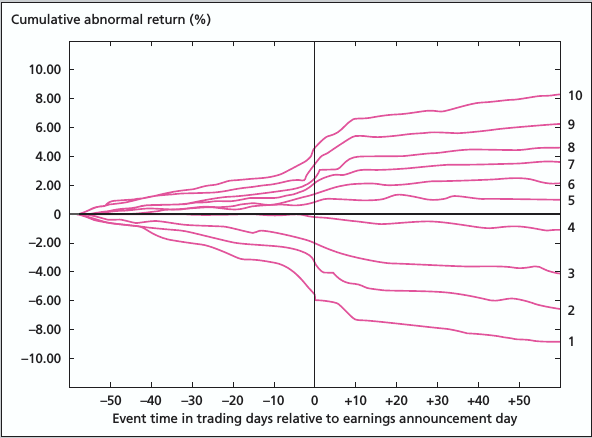
\includegraphics[width=1\linewidth]{figs/fig_gros_returns}
	\caption[Retornos anormais após anúncios de lucros.]{Retornos anormais acumulados após anúncios de lucros.\\ Fonte: Foster (1984).}
	\label{fig:figgrosreturns}
\end{figure}

O resultado mais interessante do estudo diz respeito aos movimentos dos preços das ações após a data do anúncio. Os retornos anormais acumulados de ações com surpresa positiva continuam a crescer mesmo depois do anúncio de lucros se tornar público, enquanto as empresas com surpresa negativa continuam a sofrer retornos anormais negativos. O mercado parece se ajustar às informações de ganhos apenas gradualmente, resultando em um período sustentado de retornos anormais. Desta forma, seria possível obter lucros anormais simplesmente esperando por anúncios de ganhos e comprando uma carteira de ações de empresas com lucros anunciados acima dos previstos. Esses são precisamente os tipos de tendências  previsíveis que deveriam ser impossíveis em um mercado eficiente.

Algumas pesquisas sugerem que o desvio pós-anúncio nos preços de ações pode estar relacionado aos custos de negociação. Eles também apontam que retornos anormais pós-anúncio são maiores para empresas menores, para as quais os custos de negociação são mais elevados. Ainda assim, esses resultados não explicam totalmente esta anomalia. Embora os custos de negociação possam explicar a existência de desvios após os anúncios, eles não explicam por que o retorno anormal total é maior para empresas com maiores surpresas de lucros.

\section{Ineficiência versus Prêmio de Risco}

Como devem ser interpretados todos estes estudos que sugerem grandes ineficiências no mercado? Simples regras para formação de portfólios que batem o mercado, são ineficiências ou os retornos em excesso são resultado de prêmios recebidos pelo risco maior incorrido? Em todas estas estratégias que rendem lucros aumentados, caso o risco inerente a estas também seja mais alto, o investidor está apenas recebendo seu justo retorno ajustado ao risco e não verdadeiramente um lucro anormal, e portanto estaria de acordo com a atual hipótese de eficiência dos mercados.

\citeonline{Fama1993} argumentam que essas anomalias podem ser explicadas como manifestações de prêmios de risco. Utilizando uma abordagem de precificação de equilíbrio por arbitragem eles mostram que ações com maior sensibilidade aos fatores tamanho ou patrimônio/preço têm retornos médios mais altos e interpretam esses retornos como evidência de um prêmio de risco associado a esses fatores. Fama e French argumentam que o chamado modelo de três fatores, em que o risco é determinado pela sensibilidade de uma ação para: (1) a carteira de mercado (beta de mercado), (2) uma carteira que reflete os retornos relativos de pequenas e grandes empresas e, (3) um portfólio que reflita os retornos relativos de empresas com índices altos versus baixos de valor contábil (patrimônio) sobre preço, faz um bom trabalho ao explicar os retornos de ativos. Embora os índices de tamanho ou de patrimônio/preço, por si só, não sejam fatores de risco, talvez possam servir como \emph{proxies} para determinantes mais fundamentais do risco. Fama e French argumentam que esses padrões de retorno podem, portanto, ser consistentes com um mercado eficiente, no qual os retornos esperados são consistentes com o risco.

Uma interpretação oposta é oferecida por \citeonline{Lakonishok1994}, que argumentam que esses fenômenos são evidências de mercados ineficientes, mais especificamente, de erros sistemáticos nas previsões dos analistas do mercado de ações. Eles apresentam evidências de que os analistas extrapolam o desempenho passado muito para o futuro e, portanto, superestimam empresas com desempenho recentes bons e subprecificam aquelas com desempenho recente ruim.

\chapter{A Crítica Comportamentalista}
\label{cap:comportamental}

Os grandes pioneiros do estudo das finanças comportamentais foram os pesquisadores
Daniel Kahneman e Amos Tversky. Ambos foram co-autores de diversos trabalhos na área, que
incentivaram o aprofundamento do estudo da psicologia dentro da alocação de recursos na
economia.

Os primeiros trabalhos surgiram na década de 70, tentando modelar o comportamento dos investidores e quais eram as principais armadilhas psicológicas que afetavam a tomada de decisão. Dentre os principais pontos levantados pelos pesquisadores, estão:

\begin{itemize}
	\item Heurísticas de representatividade
	\item Disponibilidade
	\item Efeito ancoragem
\end{itemize}
 
Para Kahneman e Tversky, os investidores sofrem do problema de representatividade. Isto significa que, para estimar cenários de probabilidade, normalmente são utilizadas heurísticas na tomada da decisão, que acabam desviando da real representação desejada. Heurísticas são
fatores simplificadores de pensamento: formas de padronizar e estereotipar comportamentos para facilitação da compreensão.

A disponibilidade é um conceito que trata sobre como informações recentes influenciam no julgamento das probabilidades e predições. Desta forma, são gerados vieses que deslocam a análise do real valor. É um ponto importante que fundamentou a pesquisa de inúmeros comportamentalistas, como Werner F. M. De Bondt e Richard Thaler, que trataram da hipótese das reações exageradas e que é o próximo conteúdo a ser comentado no trabalho.

Kahneman e Tversky também descobriram o chamado efeito ancoragem,  em que tomadores de decisão são influenciados por uma “base” ou “valor inicial”; ou seja, também é possível criar vieses a partir de valores e informações que fogem da ideia fundamental. Desta forma, ambos os pesquisadores solidificaram a introdução do comportamento humano afetando a tomada de decisão na alocação de recursos, abrindo caminho para ideias complementares na hipótese dos mercados eficientes.

\section{Hipótese das reações exageradas}

\citeonline{Bondt1985}, descobriram que os preços das ações reagem de forma exagerada, evidenciando características de um mercado fracamente eficiente. Este documento marcou o início das finanças comportamentais.

Ambos defendem a ideia de que os agentes econômicos dão um peso maior para as informações mais recentes, fazendo com que flutuações diárias tenham grande influência na tomada de decisão dos gestores. Esta ideia é fortalecida por \citeonline{Shiller1981}, que defende que as flutuações dos mercados não são compatíveis com a incidência de pagamento de dividendos. Ou seja, os movimentos nos preços não são racionais pois fogem do real valor dos ativos, que deriva da reação exagerada dos agentes em relação aos acontecimentos. Assim, “investidores têm a tendência de dar uma importância desproporcional a eventos econômicos de curto prazo”.

Assim, um questionamento surge: quais são as condições de equilíbrio para mercados no qual alguns agentes não possuem comportamento racional, no sentido de não revisar as suas expectativas? Para isso, Bondt e Thaler desenvolveram alguns testes empíricos para tal. No caso de uma mudança súbita nos preços de ativos do mercado acionário, Bondt e Thaler chegaram a duas hipóteses: 

\begin{itemize}
	\item Movimentos extremos nos preços vão ser seguidos por uma por um movimento contrário ao do choque; 
	\item Quanto maior for o choque nos preços, maior será o ajuste seguinte.
\end{itemize}

Ambas hipóteses violam a forma fraca de eficiência de mercado. Assim, os pesquisadores tiveram o objetivo de testar se as hipóteses de reações exageradas em flutuações de curto prazo são previsíveis. Para isso, Bondt e Thaler separaram portfólios de ações em duas categorias: os “vencedores” e os “perdedores”.

Tendo os retornos acumulados de várias ações, eles formaram portfólios com ações que obtiveram retornos entre os 10\% melhores (quantil 90\%), que foram classificados como os vencedores, e os portfólios que ficaram ações com retornos entre os 10\% piores (quantil 10\%) foram classificados como os perdedores. Assim, como foi o comportamento visto no retorno destes portfólios montados nos meses seguintes? Bondt e Thaler usaram a abordagem do CAR (cumulative average residual).

\begin{figure}[h]
	\centering
	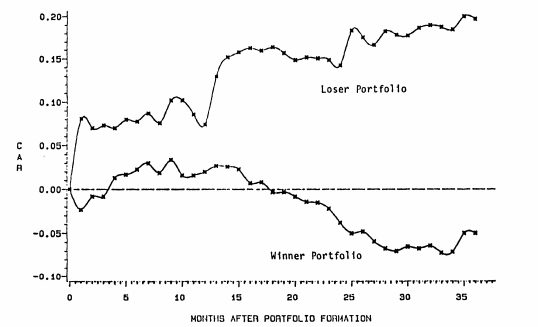
\includegraphics[width=1\linewidth]{figs/fig_comp_winner}
	\caption[Retornos de portfólios vencedores e perdedores]{Retornos residuais de portfólios formados com ações vencedoras e perdedoras.\\ Fonte: \citeonline{Bondt1985}}
	\label{fig:figcompwinner}
\end{figure}

Os resultados dos testes se encaixaram na teoria da hipótese de reações exageradas. Portfólios com ações do quantil 10\% performaram em até 19.6\%, em média dos 36 meses seguintes, que o mercado. Já os portfólios vencedores, do quantil 90\%, performaram em média 5\% abaixo do mercado. Assim, o módulo da diferença entre os portfólios vencedores e perdedores ficou em 24.6\%.

Assim, algumas evidências foram encontradas:

\begin{itemize}
	\item O efeito de reação exagerada é assimétrico: é muito maior para os perdedores que para os vencedores;
	\item Boa parte dos retornos excessivos vêm no mês de janeiro (melhores perspectivas de um novo ano, quem sabe?
\end{itemize}

\section{Estratégias que buscam valor}

\citeonline{Lakonishok1994}, fornecem evidências de que as estratégias de valor geram retornos mais altos porque essas estratégias exploram o comportamento sub-ótimo do investidor típico e não porque estas são fundamentalmente mais arriscadas.Essas estratégias de valor são contrárias às estratégias “ingênuas”, que podem ir desde dar muita importância a retornos passados até ter reações exageradas em relação a notícias más ou boas; assim, obteriam melhores retornos.
Em uma menção a hipótese das reações exageradas, Lakonishok diz que os gestores que “apostam contra” esta visão ingênua obtém melhores retornos pois investem desproporcionalmente em ações que estão subvalorizadas e investem menos em ações supervalorizadas. Assim, seria possível que alguns investidores “batessem o mercado”.

\citeonline{Kahneman1982} explicam que predições intuitivas são, tipicamente, não regressivas: pessoas comumente fazem predições com informações cuja validade preditiva e confiabilidade são questionáveis, como se ancorar em dados passados que tiveram ótimo desempenho (que em algum momento regredirão à média). Assim, investidores poderiam bater os ingênuos vendendo ações que tiveram grande desempenho passado e com grandes expectativas de retorno para o futuro e, do outro lado, comprar ações com baixos retornos passados e com poucas expectativas de retornos para o futuro. Desta forma, é aproveitado o conceito de reversão à média para projeções de retornos.

Tendo os chamados “investidores contrários” obtido melhores retornos ao longo do tempo, surge a pergunta: seriam as suas estratégias mais arriscadas? Seria esse o motivo dos melhores retornos? Duas teorias foram propostas para explicar porque estratégias de valor produziram melhores retornos. A primeira diz que os investidores contrários/de valor exploraram os erros dos investidores ingênuos; a segunda teoria diz que eles poderiam estar mais expostos ao risco.

Para isso, dois conceitos são importantes neste estudo: 

\begin{itemize}
	\item As ações de valor são aquelas com baixo desempenho passado e com pouca esperança de retornos no longo prazo no ponto de vista dos investidores (que já citamos parágrafos acima);
	\item As ações “glamorosas”: são aquelas com alto desempenho passado e com grandes expectativas de retornos para o futuro.
\end{itemize}

\begin{figure}
	\centering
	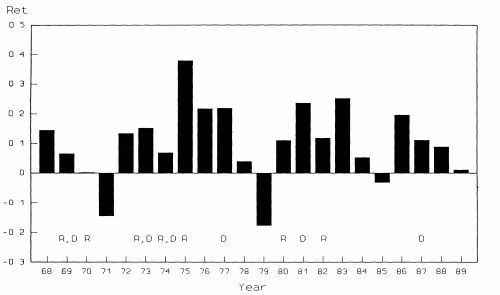
\includegraphics[width=1\linewidth]{figs/fig_comp_value}
	\caption[Retornos de estratégias Valor versus Glamor]{Retornos de estratégias Valor versus Glamor.\\ Fonte: \citeonline{Lakonishok1994}.}
	\label{fig:figcompvalue}
\end{figure}

Na figura \ref{fig:figcompvalue}, vemos a diferença entre os retornos das ações de “valor” e retornos das ações de “glamour”. Em apenas três anos dentre a série estudada esta relação foi negativa, ou seja, com ações glamorosas tendo melhor desempenho. No final, a conclusão foi de que, visto que os dados de crescimento de fluxo de caixa e outros tipos de dados das empresa foram muito menores que o esperado pelo mercado, foi entendido que os agentes superestimaram consistentemente estas “empresas glamorosas”. Uma das propostas foi de que as ações de valor apresentaram maior risco, o que foi desmentido: os indicadores fundamentais de análise de risco mostraram pouca diferença entre as ações de “valor” para as ações “glamour”.

\section{Psicologia, arbitragem e mercado eficientes}

Para \citeonline{Sharpe1990}, o conceito fundamental de arbitragem é de negociações simultâneas de compra e venda de um ativo essencialmente similar ou igual em dois diferentes mercados, ganhando na diferença de preços. Além disso, para \citeonline{Shleifer1997}, a arbitragem tem um papel crucial em levar os preços para o seu valor fundamental e para manter os mercados eficientes. Dada a importância da arbitragem na teoria dos mercados eficientes, como o comportamento dos agentes econômicos afeta o papel da arbitragem?

No modelo de arbitragem implícita de \citeonline{Fama1965}, ele assume a hipótese de um mercado com um número gigantesco de pequenos “arbitradores”, cada um tomando uma posição infinitesimal contra o descolamento de preços do valor fundamental em uma variedade de mercados. Também, como as suas posições são pequenas, falta de capital não é um problema e os arbitradores são neutros em relação ao risco. Assim, na coletividade das ações de todos os agentes, os preços voltariam para o valor fundamental. Porém, para \citeonline{Shleifer1997}, um dos maiores problemas deste modelo é de que geralmente, estes pequenos arbitradores não são os agentes que possuem conhecimento e informação para atuar com arbitragem; geralmente, a arbitragem é conduzida relativamente por pouco profissionais, extremamente especializados.

A crítica de que a arbitragem não é perfeitamente eficiente para levar os mercados à eficiência é a de que os arbitradores podem sofrer da aversão ao risco dos parceiros, aqueles que lhe confiam para gerir os seus investimentos. Ao contrário de arbitradores que utilizam do próprio capital para a alocação de recursos e se baseiam no retorno esperado das negociações, os investidores, por outro lado, podem alocar os seus investimentos baseados no retorno passado dos arbitradores. Assim, em momentos que o arbitrador precisasse de mais recursos por já estar totalmente posicionado, ele não teria esse suporte e, assim, perder as melhores oportunidades de descolamento de preços. Além disso, o acontecimento deste cenário também afeta o comportamento do arbitrador, que ficará mais cauteloso em fazer suas negociações. A conclusão: o arbitrador não conseguirá sempre ter uma ação racional e, com isso, a arbitragem se torna menos eficiente para fazer o mercado alcançar a sua eficiência.


\chapter{Gestão de Portfólios}
\label{cap:gestao}

Esforços casuais para selecionar ações provavelmente não serão recompensados. A competição entre os investidores garante que qualquer técnica de avaliação de ações facilmente implementada será usada de maneira suficientemente ampla para que qualquer percepção extra derivada desta análise seja refletida nos preços das ações. Somente análises sérias e técnicas incomuns podem gerar o discernimento diferencial necessário para gerar lucros econômicos. Além disso, essas técnicas são economicamente viáveis apenas para gestores de grandes carteiras. Se você tem apenas R\$ 100.000 para investir, mesmo uma melhora de 1\% ao ano no desempenho gera apenas R\$ 1.000, não o suficiente para justificar grandes esforços. O gestor de um fundo de 100 milhões, no entanto, colheria um lucro extra de R\$ 1 milhão anualmente para o mesmo incremento de 1\%.

A hipótese do mercado eficiente prevê que mesmo uma análise fundamentalista acrescentará pouco valor. Se os analistas confiarem nos lucros publicamente disponíveis e nas informações do setor, a avaliação de um analista sobre as perspectivas da empresa provavelmente não será significativamente mais precisa que a de outros. Existem muitas empresas bem informadas e bem financiadas que conduzem essa pesquisa de mercado e, diante dessa concorrência, será difícil descobrir dados que também não estão disponíveis para outros analistas. Somente analistas com uma visão única seriam recompensados.

A análise fundamentalista é muito mais difícil do que simplesmente identificar empresas bem administradas e com boas perspectivas. A descoberta de boas empresas não traz lucros em excesso ao investidor se o resto do mercado também sabe que essas empresas são boas. Se o conhecimento já for público, o investidor será forçado a pagar um alto preço por essas empresas e não obterá uma taxa de retorno superior. É por isso que a análise fundamentalista é difícil. Não é suficiente fazer uma boa análise de uma empresa, você pode ganhar dinheiro (ajustado ao risco) somente se sua análise for melhor do que a de seus concorrentes, porque o preço de mercado deve refletir todas as informações normalmente disponíveis.

Os proponentes da hipótese do mercado eficiente acreditam que a administração ativa de portfólios é em grande parte um esforço desperdiçado e é improvável que justifique as despesas incorridas. Por isso, eles defendem uma estratégia de investimento passiva que não faz nenhuma tentativa de superar o mercado. Uma estratégia comum para o gerenciamento passivo é criar um fundo de índice, que é um fundo projetado para replicar o desempenho de um amplo índice de ações.

Um princípio básico na seleção de portfólio é a diversificação. Mesmo que todas as ações tenham um preço justo, cada uma delas ainda representa um risco específico da empresa, que pode ser eliminado por meio da diversificação. Portanto, a seleção racional de ativos, mesmo em um mercado eficiente, exige a seleção de um portfólio cuidadosamente diversificado. Além disso, essa carteira deve fornecer o nível de risco sistemático que o investidor deseja. Mesmo em um mercado eficiente, os investidores devem escolher os perfis de risco-retorno que considerem apropriados.

Do ponto de vista da gestão de carteiras, a questão da eficiência do mercado resume-se a se os investidores profissionais podem obter lucros econômicos anormais consistentes. O melhor teste é simplesmente olhar para o desempenho dos profissionais de mercado e ver se o seu desempenho é superior ao de um fundo de índice passivo que compra e detém uma carteira de mercado. As evidências não apoiam a afirmação de que carteiras administradas profissionalmente podem consistentemente vencer o mercado. Por outro lado, há algumas evidências fracas de persistência no desempenho, o que significa que os melhores gestores em um período tendem a continuar sendo melhores nos períodos seguintes. Tal padrão sugere que estes gestores podem, com alguma consistência, superar seus concorrentes e seria incompatível com a noção de que os preços de mercado já refletem todas as informações relevantes.

Como primeiro teste, podemos examinar os retornos ajustados ao risco (ou seja, o alfa, ou o retorno em excesso do retorno exigido com base no beta de mercado em cada período) de uma grande amostra de fundos mútuos. \citeonline{Malkiel1995}, calcula estes retornos anormais para uma grande amostra de fundos mútuos entre 1972 e 1991. Os resultados, que aparecem na figura \ref{fig:figgrosalphas}, mostram que a distribuição de alfas é aproximadamente em forma de uma normal, com uma média que é ligeiramente negativa, mas estatisticamente indistinguível de zero. 

Um artigo brasileiro de \citeonline{Castro2009} promove um estudo semelhante e compara o alfa gerado por fundos ativos e passivos no Brasil. Eles chegam a conclusão que após os custos, apenas 4,8\% dos fundos ativos possuem alfas positivos estatisticamente significativos, sendo que na média, os fundos ativos não geram retornos em excesso aos seus investidores. Refletem que seus achados estão de acordo com a formulação de eficiência de Jensen, onde os mercados são eficientes até o ponto onde os benefícios marginais de aquisição e atuação sobre informações se igualam aos custos marginais.

\begin{figure}[h]
	\centering
	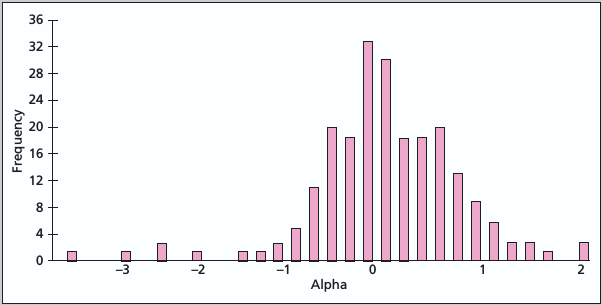
\includegraphics[width=1\linewidth]{figs/fig_gros_alphas}
	\caption[Alfas gerados por fundos americanos.]{Distribuição de alfas gerados por fundos americanos.\\ Fonte: Malkiel (1995)}
	\label{fig:figgrosalphas}
\end{figure}

Assim, as evidências sobre o desempenho ajustado ao risco dos gestores profissionais são, na melhor das hipóteses, mistas. Concluímos que o desempenho dos gestores profissionais é amplamente consistente com a eficiência do mercado. Os montantes pelos quais os gestores profissionais, enquanto grupo, batem ou não o mercado, caem na margem da incerteza estatística.

Em suma, há um papel para o gerenciamento de portfólio mesmo em um mercado eficiente. As posições ideais dos investidores variam de acordo com fatores como idade, aversão ao risco e emprego. O papel do gestor de carteira em um mercado eficiente é adequar o portfólio a essas necessidades, em vez de tentar superar o mercado.



%\chapter{Testes Empíricos}
\label{cap:testes}

\citeonline{Bollerslev1992b}

\lipsum[81]
\chapter*{Conclusões}\label{cap:conclusao}
\addcontentsline{toc}{chapter}{Conclusão}

Nos mercados financeiros, a HME é respeitada, mas não é cultuada. É reconhecido que os mercados provavelmente serão eficientes na maior parte do tempo, mas não o tempo todo. Ineficiências podem surgir particularmente durante períodos de importantes mudanças institucionais e tecnológicas. Não é possível saber com antecedência quando e onde as ineficiências do mercado surgem - mas acredita-se que elas surgirão de tempos em tempos. Os operadores do mercado adoram a volatilidade, pois sinalizam notícias e mudanças e são acompanhadas de possibilidades de lucro a serem exploradas. A identificação da previsibilidade explorável tende a ser totalmente diversificada nos mercados de títulos, ações e câmbio. Desalinhamentos entre mercados para diferentes ativos e em diferentes países geralmente apresentam as oportunidades mais importantes. Exemplos incluem arbitragem estatística e macro-arbitragem globais.

Da parte comportamentalista, podemos ver que os pesquisadores não buscam refutar a hipótese dos mercados eficientes, mas sim de poder complementar o viés psicológico dentro dos modelos de alocação de recursos. Em algumas situações em específico, o comportamento humano se torna irracional, o que faz com que os mercados não se ajustem ao valor fundamental de forma adequada. Assim, as finanças comportamentais entram na análise de mercados eficientes como forma de agregar mais complexidade e fatores de impacto no que se trata de alocação de recursos.

A recente literatura financeira parece produzir muitas anomalias de retorno a longo prazo. No entanto, as evidências não sugerem que a eficiência do mercado deva ser abandonada. Consistente com a hipótese de eficiência de mercado de que as anomalias são resultados aleatórios, a aparente reação exagerada dos preços das ações à informação é tão comum quanto a sub-reação. E a continuação de retornos anormais pré-evento é tão frequente quanto a reversão pós-evento.

A maior parte da evidência sugere que qualquer estratégia de investimento supostamente superior deve ser vista com um tanto de ceticismo. O mercado é competitivo o suficiente para que apenas informações ou percepções ligeiramente superiores ganhem dinheiro. As escolhas fáceis foram escolhidas. No final, é provável que a margem de superioridade que qualquer administrador profissional pode adicionar seja tão pequena que apenas o teste estatístico não seja capaz de detectá-la.



% ----------------------------------------------------------
% ELEMENTOS PÓS-TEXTUAIS (Referências, Glossário, Apêndices)
% ----------------------------------------------------------
%\postextual

% Referências bibliográficas
\bibliography{library}

% Glossário (Consulte o manual)
%\glossary

% Apêndices
%% ----------------------------------------------------------
% Apêndices
% ----------------------------------------------------------

% ---
% Inicia os apêndices
% ---
\begin{apendicesenv}

% Imprime uma página indicando o início dos apêndices
\partapendices

% ----------------------------------------------------------
\chapter{Primeiro Apêncice}
% ----------------------------------------------------------

\lipsum[50] % Texto qualquer. REMOVER!!

% ----------------------------------------------------------
\chapter{Perceba que o texto do título desse segundo apêndice é bem grande}
% ----------------------------------------------------------
\lipsum[51-53] % Texto qualquer. REMOVER!!

\end{apendicesenv}
% ---

% Anexos
%% ----------------------------------------------------------
% Apêndices
% ----------------------------------------------------------

% ---
% Inicia os anexos
% ---
\begin{anexosenv}

% Imprime uma página indicando o início dos anexos
\partanexos

% ---
\chapter{Nome do Primeiro Anexo}
% ---
\lipsum[30] % Texto qualquer. REMOVER!!

% ---
\chapter{Nome de Outro Anexo}
% ---

\lipsum[32] % Texto qualquer. REMOVER!!

\end{anexosenv}

% Índice remissivo (Consultar manual)
%\phantompart
%\printindex

\end{document}
